%% LyX 2.1.3 created this file.  For more info, see http://www.lyx.org/.
%% Do not edit unless you really know what you are doing.
\documentclass{report}
\usepackage[utf8]{luainputenc}
\usepackage[a4paper]{geometry}
\geometry{verbose}
\setcounter{secnumdepth}{3}
\setcounter{tocdepth}{3}
\usepackage{amsmath}
\usepackage{amssymb}
\usepackage{graphicx}
\usepackage[unicode=true,
 bookmarks=false,
 breaklinks=false,pdfborder={0 0 1},backref=section,colorlinks=false]
 {hyperref}

\makeatletter
%%%%%%%%%%%%%%%%%%%%%%%%%%%%%% User specified LaTeX commands.
\usepackage{framed}
\usepackage[outerbars]{changebar}

\makeatother

\begin{document}

\title{Notes}


\author{Léo}

\maketitle
While being self-sufficient, those notes focus on the recent results
in optimization and don't pretend to be an exhaustive review of optimization
methods.


\chapter{Music generation}


\chapter{Orchestral inference}


\section{Projective symbolic orchestration}


\subsection{Factored Gated Conditional RBM}

The two next steps should be easy to implement and imply important
changes : 
\begin{itemize}
\item take dynamics into consideration 
\item event level 
\end{itemize}
Other leads should be quickly investigated, although not spending
to much time on it 
\begin{itemize}
\item Greatly increase the number of factor units. It should greatly improve
the \textquotedbl{}expressiveness\textquotedbl{} of the network. 
\end{itemize}

\section{Multi-modal signal/symbolic networks}

The idea is to build a system where orchestration is controlled in
real-time by a set of faders which in they turn control some spectral
features. It would be a purely generative system that would not rely
on a piano score, but instead would be more an ambient generator (I
imagine the result as \textquotedbl{}sound layers\textquotedbl{}).


\subsection{Learning step}

\begin{figure}
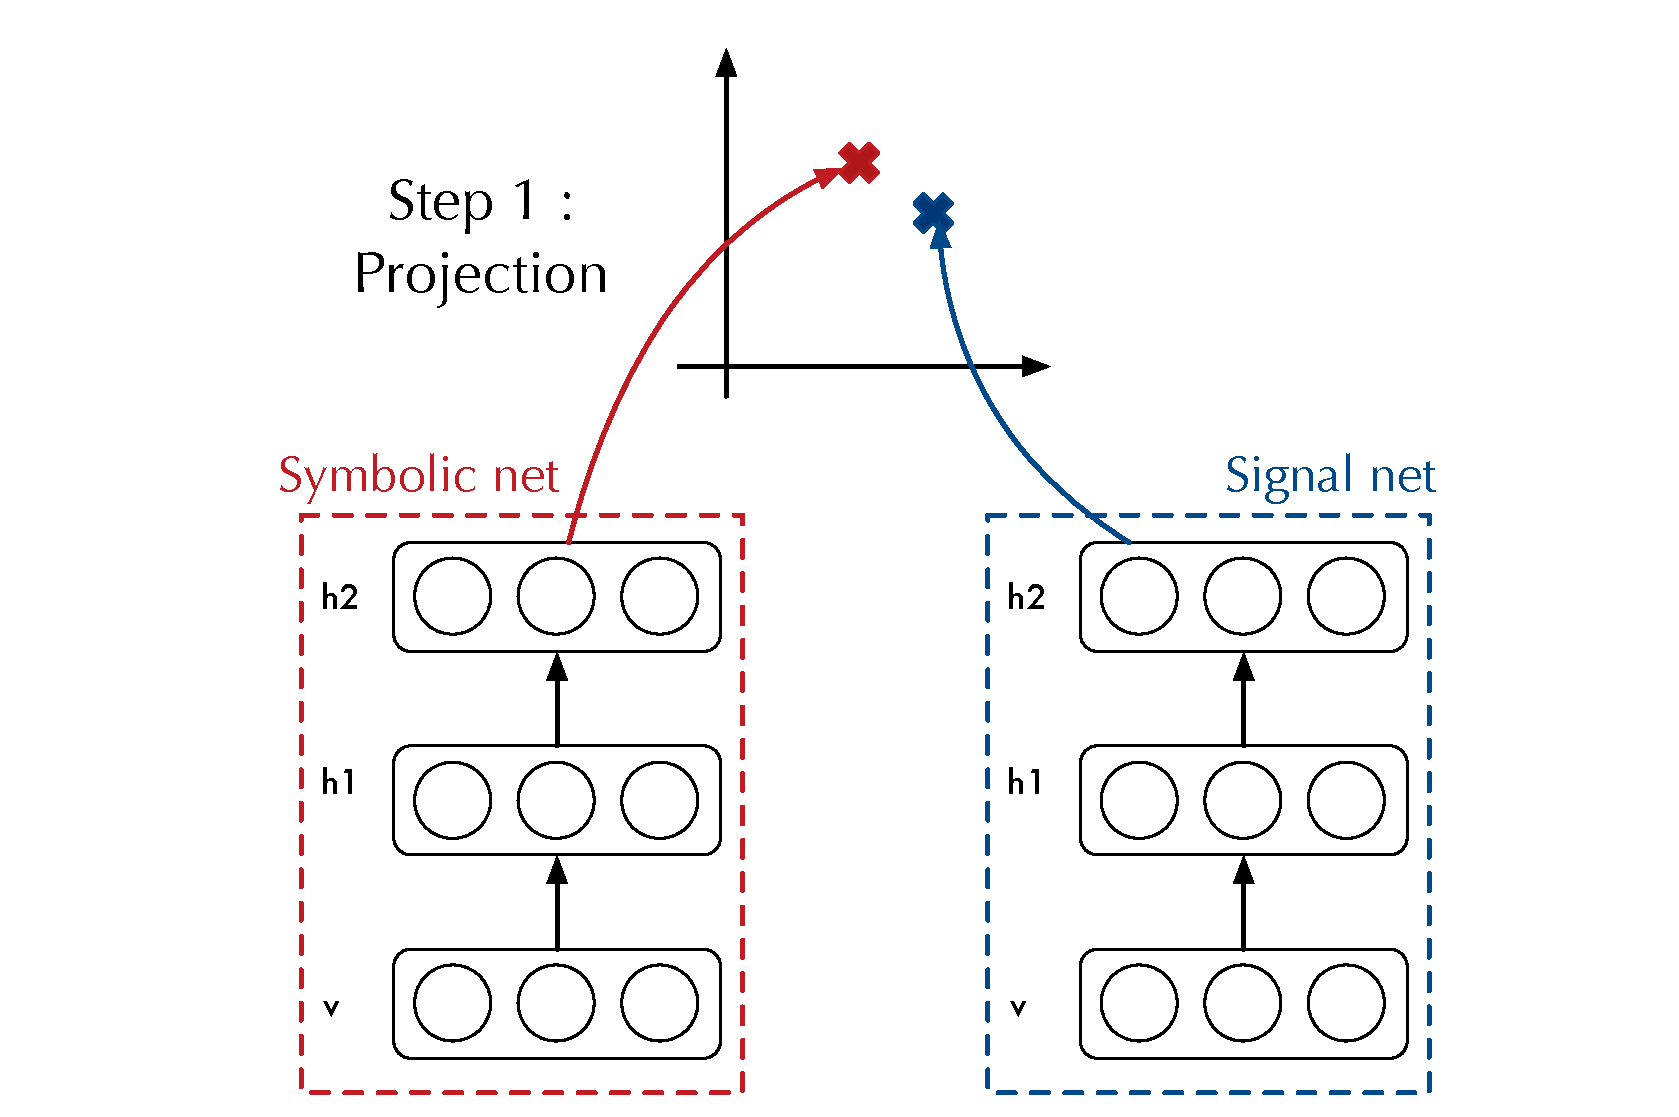
\includegraphics[width=0.47\paperwidth]{/Users/leo/Documents/Mega_sync/Travail/Recherche/GitHub_Aciditeam/documents/figures/Multimodal/siamese_net_projection}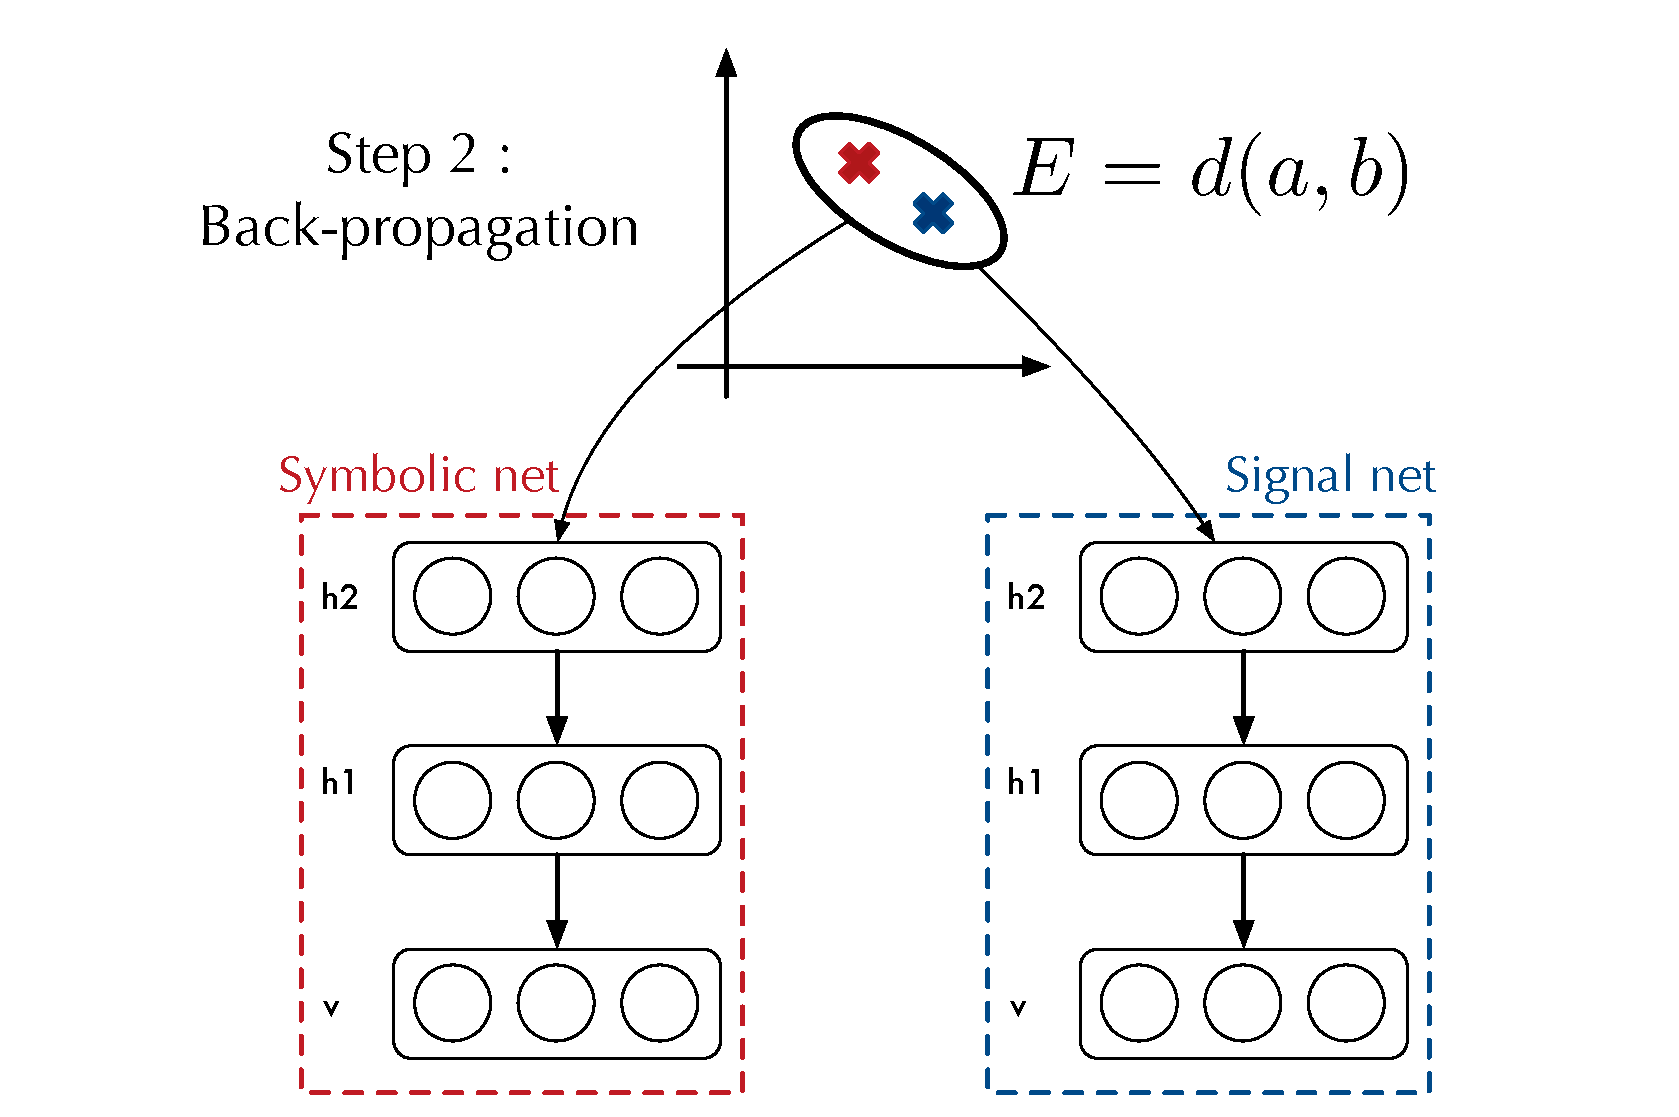
\includegraphics[width=0.47\paperwidth]{/Users/leo/Documents/Mega_sync/Travail/Recherche/GitHub_Aciditeam/documents/figures/Multimodal/siamese_net_backprop}

\protect\caption{Embedding of different representations in a common modal space. This
is the encoding step}


\end{figure}


The learning step rely on an orchestral database composed of the scores
(xml preferably, midi otherwise) and a recording. Each track is divided
in (short) time frames (both score and recording). The two Siamese
networks respectively receive in input a symbolic frame and its corresponding
signal frame (or its FFT, or any other perceptually relevant transformation).
The training is then divided in two steps 
\begin{enumerate}
\item unsupervised step, in order to learn relevant features in the last
layer 
\item supervised step in order to force the output of the two networks to
be close in a metric space. 
\end{enumerate}
The structure of the two networks have to be determined (recurrent
nets or simple deep architectures ? Stacked memory ?), but the first
step would rely on state of the art methods in automatic features
extraction. A first remark for the second step is that it requires
the two networks to have the same number of output units $|O|$. Those
two sets of output units define two points in $\left[0,1\right]{|O|}$
(or $\mathbb{R}_{+}^{|O|}$ if we use a different type of unit for
the output ?). The distance between those two points then define an
error function that we can differentiate in order to fine-tuned the
two networks with back-propagation.


\subsection{Generation step}

\begin{figure}
 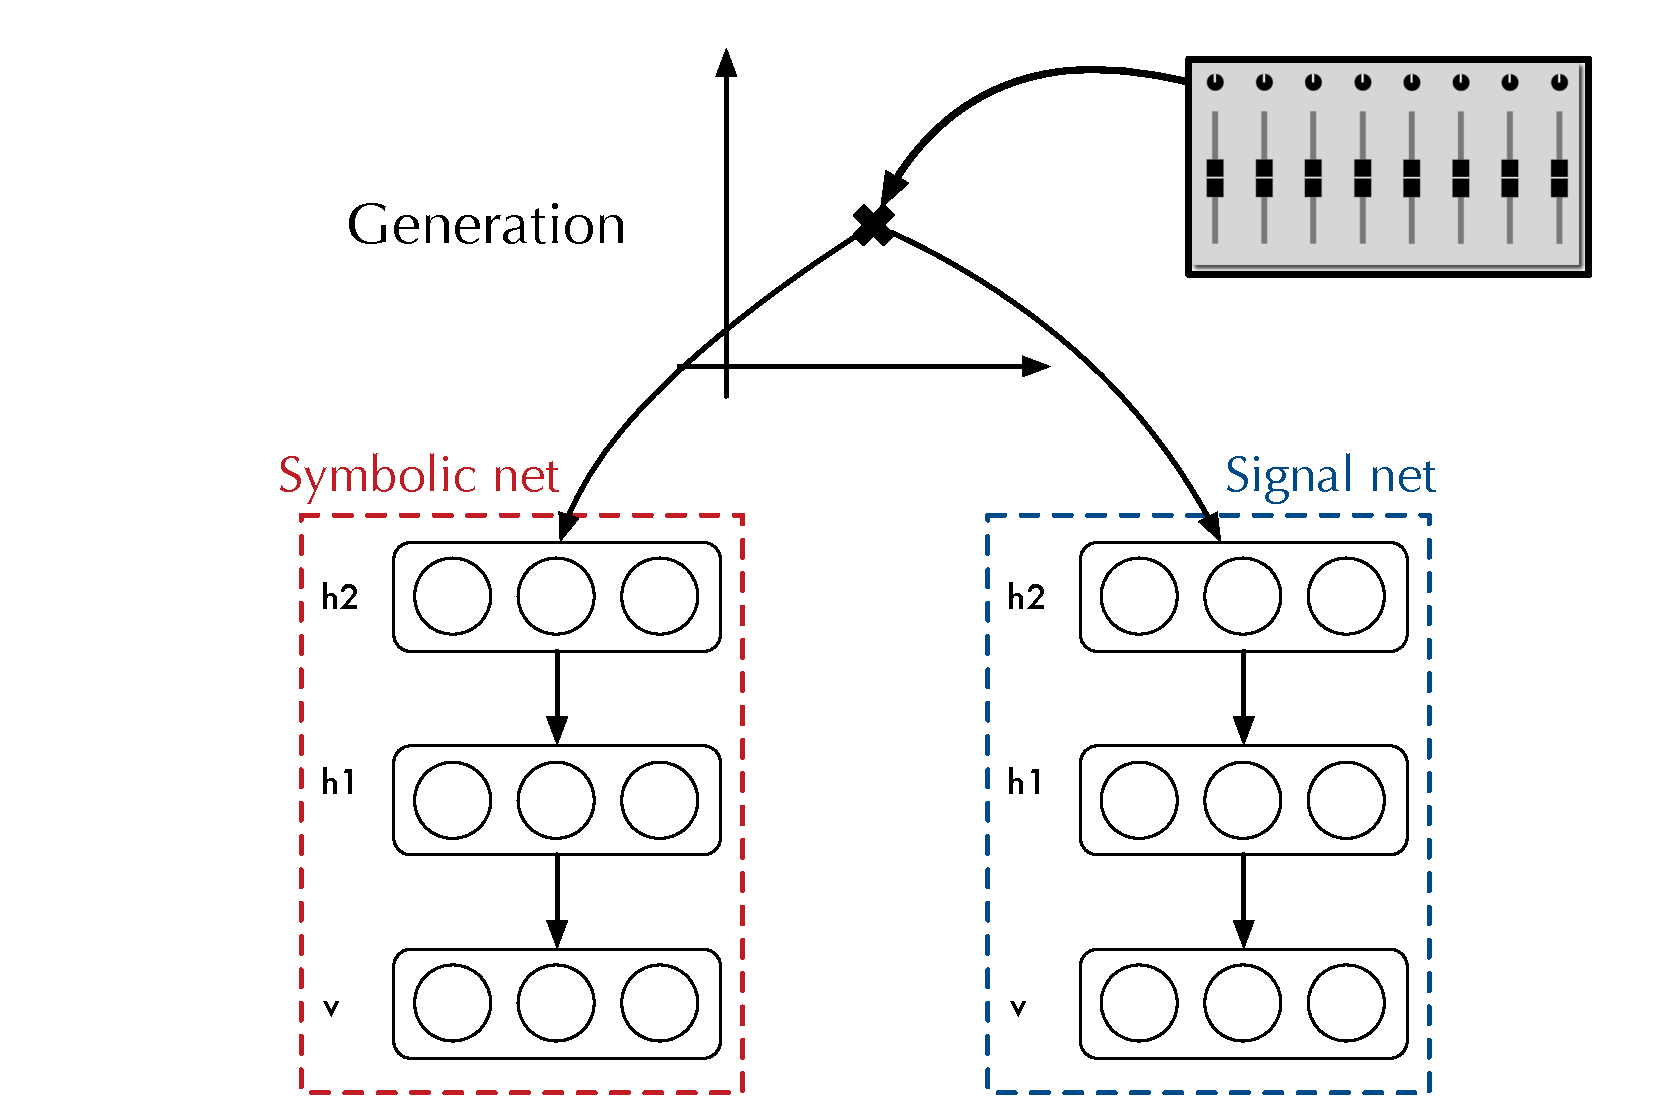
\includegraphics[width=0.97\linewidth]{/Users/leo/Documents/Mega_sync/Travail/Recherche/GitHub_Aciditeam/documents/figures/Multimodal/siamese_net_generation}
\protect\caption{Generation step in the Siamese network.}
\end{figure}


A fader is associated to each dimensions of our \textquotedbl{}projection\textquotedbl{}
space (space defined by the output units). The position of each fader
then define the coordinate of the synthesis point. We associate to
each output unit the value of each coordinate of the synthesis point
and back-propagate those values in the \textquotedbl{}symbolic\textquotedbl{}
network to obtain the orchestration and in the \textquotedbl{}spectral\textquotedbl{}
network to observe the ideal signal/spectrogram (probably not totally
the same that the one corresponding to the symbolic score played).


\subsection{Unsolved questions}
\begin{itemize}
\item Input for the \textquotedbl{}spectral/signal\textquotedbl{} network 
\item Which architecture ? (recurrent nets or simple deep architectures
? Stacked memory, Deep LSTM ?)
\item Which type of input \textbf{and} output units ? 
\item How to deal with continuity of orchestration ? A lead could be to
define Siamese network for past frames and force recent past to be
close to the actual frame in the projection space. 
\end{itemize}

\subsection{Application}
\begin{itemize}
\item Generating orchestration 
\item audio to score. Plus it gives a good evaluation framework. \end{itemize}

\end{document}
